\hypertarget{camerawidget_8cpp}{\section{camerawidget.\-cpp File Reference}
\label{camerawidget_8cpp}\index{camerawidget.\-cpp@{camerawidget.\-cpp}}
}


Ce programme permet la conversion d'une Ipl\-Image en une Q\-Pixmap et le placement du constructeur (widget) dans un layout.  


{\ttfamily \#include \char`\"{}camerawidget.\-h\char`\"{}}\\*
Include dependency graph for camerawidget.\-cpp\-:\nopagebreak
\begin{figure}[H]
\begin{center}
\leavevmode
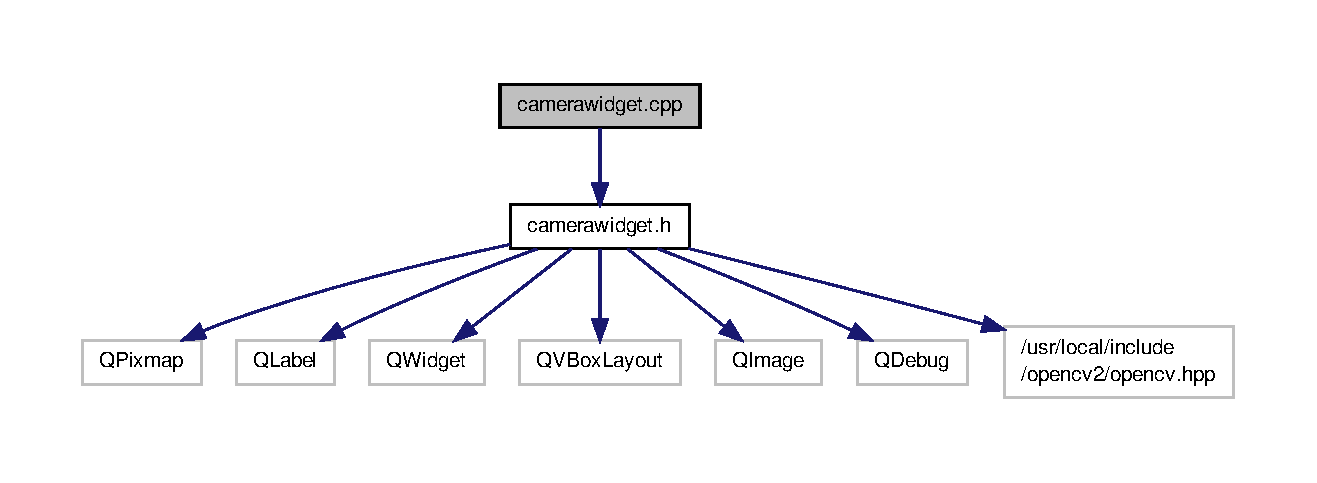
\includegraphics[width=350pt]{camerawidget_8cpp__incl}
\end{center}
\end{figure}


\subsection{Detailed Description}
Ce programme permet la conversion d'une Ipl\-Image en une Q\-Pixmap et le placement du constructeur (widget) dans un layout. \begin{DoxyAuthor}{Author}
Martin P\-R\-A\-D\-E\-A\-U 
\end{DoxyAuthor}
\begin{DoxyVersion}{Version}
Version finale 
\end{DoxyVersion}
\begin{DoxyDate}{Date}
Janvier 2014 
\end{DoxyDate}


Definition in file \hyperlink{camerawidget_8cpp_source}{camerawidget.\-cpp}.

